\section{Experiments and Results}
\label{sec:results}

\paragraph{Data.} I run the system on five hand-held phone photos of printed
monophonic scores: \emph{Yankee Doodle}, \emph{Twinkle Twinkle}, \emph{Mary Had
a Little Lamb}, a CS\,131 motif, and \emph{London Bridge}. Four images undergo
the whole pipeline; one (\emph{London Bridge}) is a failure case
(Sec.~\ref{sec:results:limits}). For classification I use a mined database of
$35{,}933$ $64\times64$ glyph crops, all sourced from clean PrIMuS, with $20\%$
held out for validation; all pitches were transcribed by hand.

\subsection{Geometry stages are robust}
\label{sec:results:geometry}
Rectification is successful on all five images: the slant on remaining staves is
$\le 0.22^{\circ}$, and border penetration is $\le 2.6\%$ on all images. My two
corner-detection approaches are sufficient across the set (Table~\ref{tab:geom}).
Staff detection then recovers every stave on the four pipeline images ($12$
staves total) at default Hough parameters, and after morphological stripping and
connected-component grouping I obtain fairly clean candidates.

\begin{table}[t]
  \centering
  \small
  \setlength{\tabcolsep}{4pt}
  \resizebox{\columnwidth}{!}{%
  \begin{tabular}{lccccc}
    \toprule
    Image & Method & Slant & Border & Staves & Symbols\\
    \midrule
    Yankee Doodle      & Hough  & $0.22^{\circ}$ & $2.6\%$ & 4 & 94\\
    Twinkle Twinkle    & PolyDP & $0.20^{\circ}$ & $0.0\%$ & 3 & 68\\
    Mary Had a Lamb    & Hough  & $0.07^{\circ}$ & $1.9\%$ & 2 & 45\\
    CS\,131 motif      & Hough  & $0.11^{\circ}$ & $1.1\%$ & 3 & 27\\
    \midrule
    \multicolumn{4}{l}{\emph{Pass rate (rectification)}} & \multicolumn{2}{c}{$5/5$}\\
    \multicolumn{4}{l}{\emph{Pass rate (staff detection)}} & \multicolumn{2}{c}{$4/4$}\\
    \bottomrule
  \end{tabular}}
  \caption{Geometry front end. Residual slant, border intrusion, detected staves,
  and segmented symbol candidates. All staves are recovered at default parameters.}
  \label{tab:geom}
\end{table}

\begin{figure*}[t!]
  \centering
  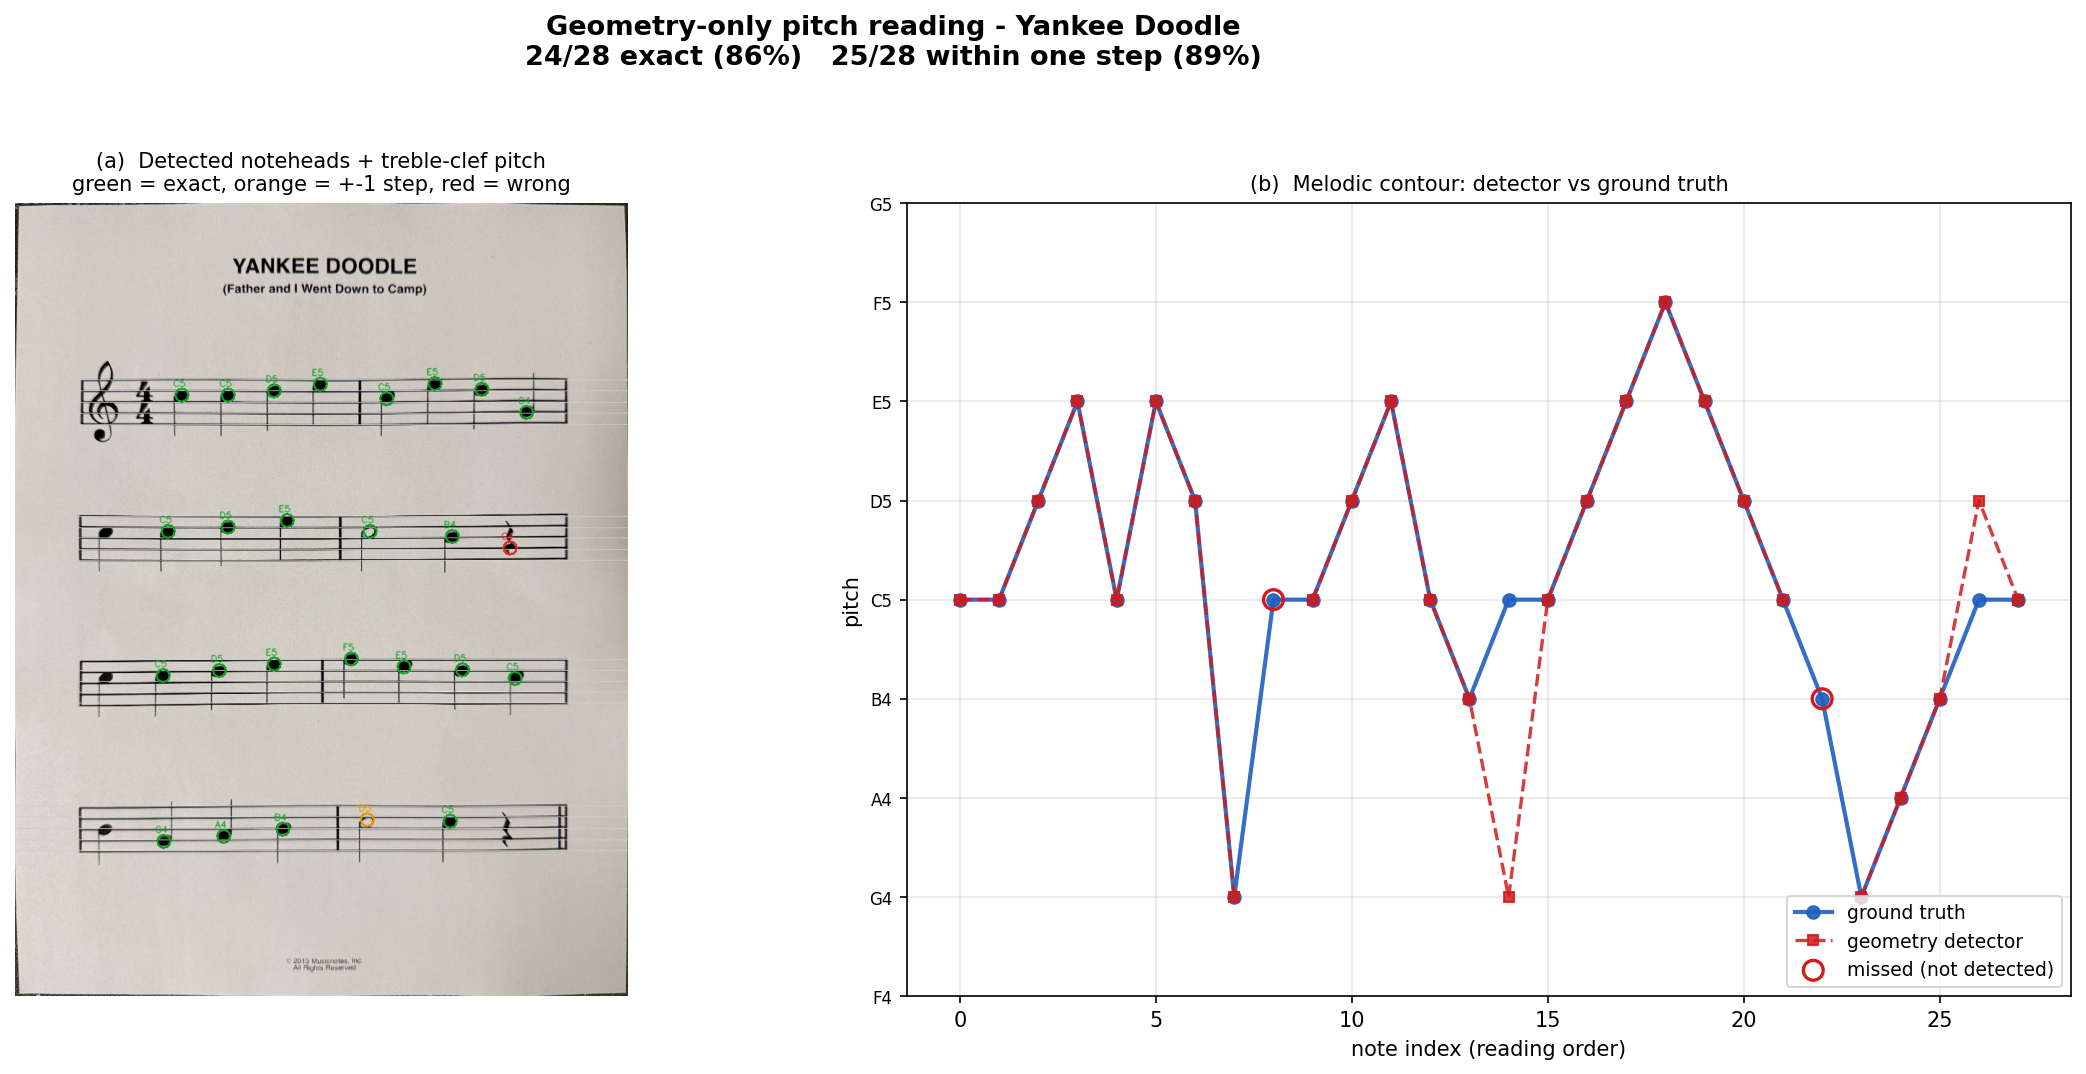
\includegraphics[width=0.44\linewidth]{figures/geometry_pitch.png}
  \caption{\textbf{Geometry-only pitch reading on \emph{Yankee Doodle}}
  (Sec.~\ref{sec:results:pitch}). Left: template-matched noteheads labelled with
  the inferred pitch (green $=$ exact, orange $=$ within one step, red $=$ wrong).
  Right: inferred melodic contour vs.\ ground truth (open circles mark the two
  undetected noteheads). The reader attains $24/28$ ($86\%$) exact and $25/28$
  ($89\%$) within one step, with no segmentation or classification.}
  \label{fig:geom_pitch}
\end{figure*}

\subsection{The clean-to-real domain gap}
\label{sec:results:gap}
The learned classifier behaves very differently on clean PrIMuS and real
photographic crops. It achieves $58.9\%$ validation accuracy on clean PrIMuS
glyphs but only $22.7\%$ accuracy on $97$ real photographic crops, a
$36.2$-point gap (Table~\ref{tab:cnn}). Class-dependent error rates reveal the
gap's scale: quarter notes are fairly robust ($24.6\%$) and eighth notes very
robust ($80\%$), but hollow half notes fail completely ($0/7$) and the residual
\emph{other} category never recovers ($0/21$). The cause is immediately apparent
from the real photo crops: the clean PrIMuS glyphs are crisp and uniform, whereas
photographic crops have blur, fractured stems, filled-in noteheads, and trace
background staff lines which the clean-trained features simply never encountered.
This is the primary insight of the paper: a system trained for appearance-based
classification on engravings does not transfer to phone photographs.

\begin{table}[t]
  \centering
  \small
  \setlength{\tabcolsep}{6pt}
  \begin{tabular}{lcc}
    \toprule
    Setting / Class & Crops & Accuracy\\
    \midrule
    PrIMuS validation (clean) & --- & $\mathbf{58.9\%}$\\
    Local phone crops (real)  & 97  & $\mathbf{22.7\%}$\\
    \midrule
    \quad note\_quarter & 57 & $24.6\%$\\
    \quad note\_eighth  & 10 & $80.0\%$\\
    \quad note\_half    & 7  & $0.0\%$\\
    \quad rest\_quarter & 2  & $0.0\%$\\
    \quad other         & 21 & $0.0\%$\\
    \midrule
    \emph{Clean-to-real gap} & & $\mathbf{-36.2}$ pts\\
    \bottomrule
  \end{tabular}
  \caption{Domain-gap study for \textsc{SymbolCNN}. A model close to $60\%$ on
  clean glyphs plunges to under $23\%$ on real-photo crops, missing its hollow and
  catch-all classes entirely.}
  \label{tab:cnn}
\end{table}

\subsection{End-to-end pitch and the geometry remedy}
\label{sec:results:pitch}
The domain gap also extends to the full pipeline. On the
segmentation-plus-classifier path, end-to-end pitch accuracy on all four pieces
is low (Table~\ref{tab:pitch}): $8$--$14\%$ exact and $17$--$50\%$ within one
step. Mistakes are due not so much to the pitch geometry of
Eq.~\eqref{eq:staffpos}---exact where the notehead is properly located---as to
upstream segmentation merges and misclassifications.

\begin{table}[t]
  \centering
  \small
  \setlength{\tabcolsep}{5pt}
  \resizebox{\columnwidth}{!}{%
  \begin{tabular}{lcccc}
    \toprule
    & \multicolumn{2}{c}{Baseline (seg.+CNN)} & \multicolumn{2}{c}{Geometry-only}\\
    \cmidrule(lr){2-3}\cmidrule(lr){4-5}
    Image & Exact & $\pm1$ & Exact & $\pm1$\\
    \midrule
    Yankee Doodle   & $14\%$ & $50\%$ & $\mathbf{86\%}$ & $\mathbf{89\%}$\\
    Twinkle Twinkle & $10\%$ & $19\%$ & --- & ---\\
    Mary Had a Lamb & $8\%$  & $23\%$ & --- & ---\\
    CS\,131 motif   & $8\%$  & $17\%$ & --- & ---\\
    \bottomrule
  \end{tabular}}
  \caption{End-to-end pitch accuracy. The seg.+CNN baseline is weak; the geometry
  reader (Sec.~\ref{sec:method:pitch}) lifts \emph{Yankee Doodle} from $14\%$ to
  $86\%$.}
  \label{tab:pitch}
\end{table}

The geometry-only reader presents a different scenario
(Fig.~\ref{fig:geom_pitch}). On \emph{Yankee Doodle} it localizes $26$ of the
$28$ noteheads and, under the standard alignment-based metric, reads $24/28$
($86\%$) pitches exactly and $25/28$ ($89\%$) within one step (a six-fold
increase over baseline). Since pitch is extracted directly from the notehead
position using Eq.~\eqref{eq:staffpos}, it is read perfectly whenever the
notehead is detected, and only two pitch-reading errors (one missed notehead pair
and one localization slip) are produced. For phone-photo OMR, geometry
generalizes where the appearance-based models trained on clean data fail.

\subsection{Diagnostics and Limitations}
\label{sec:results:limits}
It was particularly interesting to see how two approaches---overzealous
stem-bridging and over-segmentation of a glyph---resulted in failing to connect
beamed notes or completely separating a glyph. By linking the morphological
kernel size to $s$, I eliminated these problems. Another clear limit is
\emph{London Bridge}: a thick dark shadow heavily skews the page mask, so the
corner cascade returns a slanted rather than square quadrilateral, in turn
causing staff detection to fail. This highlights shadow-tolerant binarization as
future work.
